\documentclass[aspectratio=169,10pt]{beamer}

\usetheme{Madrid}
\usecolortheme{seahorse}

\usepackage{amsmath}
\usepackage{amssymb}
\usepackage{mathtools}
\usepackage{graphicx}
\usepackage{listings}
\usepackage{xcolor}

% Define custom environments for remark and exercise
\newenvironment{remark}
  {\begin{block}{Remark}}
  {\end{block}}

\newenvironment{exercise}
  {\begin{block}{Exercise}}
  {\end{block}}

\graphicspath{{figures/}}

% Code listing style
\lstset{
    basicstyle=\ttfamily\scriptsize,
    commentstyle=\color{green!50!black}\itshape,
    keywordstyle=\color{blue},
    stringstyle=\color{red},
    numbers=left,
    numberstyle=\tiny\color{gray},
    frame=single,
    breaklines=true,
    language=Python
}

\setbeamertemplate{footline}[frame number]

% Define colors
\definecolor{darkgreen}{rgb}{0,0.5,0}
\definecolor{darkblue}{rgb}{0,0,0.7}

\title[Chapter 30: Best Approximation Algorithms]{Chapter 30: Best Approximation Algorithms}
\subtitle{Convex Analysis and Monotone Operator Theory}
\author[]{Lecture Notes}
\date{\today}

\begin{document}

% ============================================================================
\begin{frame}
  \titlepage
\end{frame}

% ============================================================================
\begin{frame}{Overview}
  \tableofcontents
\end{frame}

% ============================================================================
\section{Introduction and Halper's Algorithm}
% ============================================================================

\begin{frame}{Best Approximation Problem}
  \begin{block}{Core Problem}
    Given a nonempty closed convex subset $C$ of a Hilbert space $\mathcal{H}$ and a point $x \in \mathcal{H}$, find the unique point $p \in C$ that minimizes $\|x - y\|$ over all $y \in C$.
  \end{block}

  \vspace{0.3cm}

  \begin{definition}
    For a point $x$, the \textbf{projection} onto $C$ is
    \[
      P_C x := \arg\min_{y \in C} \|x - y\|
    \]
  \end{definition}

  \vspace{0.3cm}

  \begin{itemize}
    \item Projections exist and are unique (by Hilbert space theory)
    \item $P_C$ is a nonexpansive operator: $\|P_C x - P_C y\| \leq \|x - y\|$
    \item Main goal: Design iterative algorithms converging to $P_C x$
  \end{itemize}
\end{frame}

% ============================================================================

\begin{frame}{Halper's Algorithm}
  \begin{theorem}[Halper's Algorithm]
    Let $D$ be a nonempty closed convex subset of $\mathcal{H}$, let $T: D \to D$ be a nonexpansive operator such that $C = \text{Fix } T \neq \emptyset$, and let $(\lambda_n)_n$ be a sequence in $[0,1]$ such that $\lambda_n \to 0$, $\sum_n \lambda_n = +\infty$, and $\sum_n |\lambda_{n+1} - \lambda_n| < +\infty$. Let $x_0 \in D$ and set
    \[
      (\forall n \in \mathbb{N}) \quad x_{n+1} = \lambda_n x + (1 - \lambda_n) T x_n.
    \]
    Then $x_n \to P_{\text{Fix } T} x$.
  \end{theorem}

  \vspace{0.3cm}

  Key convergence conditions:
  \begin{enumerate}
    \item Decreasing step sizes: $\lambda_n \to 0$
    \item Summability: $\sum_n \lambda_n = +\infty$
    \item Uniform boundedness: $\sum_n |\lambda_{n+1} - \lambda_n| < +\infty$
  \end{enumerate}
\end{frame}

% ============================================================================

\begin{frame}[fragile]{Halper's Algorithm: Python Implementation}
  \begin{lstlisting}
def halpers_algorithm(T, x, x0, lambda_seq, max_iter=1000, tol=1e-8):
    """
    Halper's fixed point algorithm.

    Parameters:
    -----------
    T : function
        Nonexpansive operator (fixed point operator)
    x : array
        Target point (for projection from fixed points)
    x0 : array
        Initial point
    lambda_seq : list
        Step sizes (decreasing to 0)
    """
    x_curr = np.array(x0, dtype=float)
    history = [x_curr.copy()]

    for n in range(min(max_iter, len(lambda_seq))):
        lam = lambda_seq[n]
        Tx = T(x_curr)
        x_next = lam * x + (1 - lam) * Tx

        if np.linalg.norm(x_next - x_curr) < tol:
            break

        x_curr = x_next
        history.append(x_curr.copy())

    return x_curr, np.array(history)
  \end{lstlisting}
\end{frame}

% ============================================================================

\begin{frame}{Corollary 30.2: Finite Family of Operators}
  \begin{corollary}
    Let $D$ be a nonempty closed convex subset, let $(T_i)_{i \in I}$ be a finite family of nonexpansive operators from $D$ to $D$ such that $C = \bigcap_{i \in I} \text{Fix } T_i \neq \emptyset$. Let $x \in D$ and $(\omega_i)_{i \in I}$ be real numbers in $[0,1]$ with $\sum_{i \in I} \omega_i = 1$. Let $(\lambda_n)_n$ be a sequence satisfying the conditions of Theorem 30.1. Let $x_0 \in D$ and set
    \[
      (\forall n \in \mathbb{N}) \quad x_{n+1} = \lambda_n x + (1 - \lambda_n) \sum_{i \in I} \omega_i T_i x_n.
    \]
    Then $x_n \to P_C x$.
  \end{corollary}

  \vspace{0.3cm}

  This is useful for finding projections onto intersections of convex sets!
\end{frame}

% ============================================================================

\begin{frame}{Corollary 30.3: Averaged Nonexpansive Operators}
  \begin{corollary}
    Let $D$ be a nonempty closed convex subset, let $m$ be a strictly positive integer, set $I = \{1, \ldots, m\}$, let $(T_i)_{i \in I}$ be a family of averaged nonexpansive operators from $D$ to $D$ such that $C = \bigcap_{i \in I} \text{Fix } T_i \neq \emptyset$. Let $x \in D$ and $(\lambda_n)_n$ be a sequence satisfying Theorem 30.1 conditions. Let $x_0 \in D$ and set
    \[
      (\forall n \in \mathbb{N}) \quad x_{n+1} = \lambda_n x + (1 - \lambda_n) T_1 \cdots T_m x_n.
    \]
    Then $x_n \to P_C x$.
  \end{corollary}

  \vspace{0.3cm}

  \begin{example}[Application: Cyclic projections]
    When each $T_i = P_{C_i}$ is a projection, the composite operator $P_{C_1} \cdots P_{C_m}$ achieves strong convergence to $P_C x$ where $C = \bigcap_i C_i$.
  \end{example}
\end{frame}

% ============================================================================

\begin{frame}{Linear Mean Ergodic Theorem}
  \begin{corollary}[30.5: Linear Mean Ergodic Theorem]
    Let $T \in \mathcal{B}(\mathcal{H})$ be nonexpansive and let $x \in \mathcal{H}$. Then
    \[
      \frac{1}{n+1} \sum_{k=0}^{n} T^k x \to P_{\ker(\text{Id}-T)} x.
    \]
  \end{corollary}

  \vspace{0.3cm}

  Key insight: The Cesàro average of iterates converges to the projection onto the kernel of $(I - T)$, which is the set of fixed points of $T$.

  \vspace{0.3cm}

  \begin{itemize}
    \item This provides strong convergence without requiring decreasing step sizes
    \item The convergence is in the mean (averaging)
    \item Weaker than pointwise convergence but easier to achieve
  \end{itemize}
\end{frame}

% ============================================================================
\section{Dykstra's Algorithm}
% ============================================================================

\begin{frame}{Dykstra's Algorithm: Motivation}
  \begin{block}{Problem}
    Find the projection of a point $x_0 \in \mathcal{H}$ onto the intersection of $m$ closed convex sets $C_1, \ldots, C_m$.
  \end{block}

  \vspace{0.3cm}

  Key challenges:
  \begin{enumerate}
    \item Computing $P_{C_1 \cap \cdots \cap C_m}$ directly is often difficult
    \item But projections $P_{C_i}$ onto individual sets may be easy to compute
    \item Dykstra's algorithm combines individual projections
  \end{enumerate}

  \vspace{0.3cm}

  \begin{figure}
    \centering
    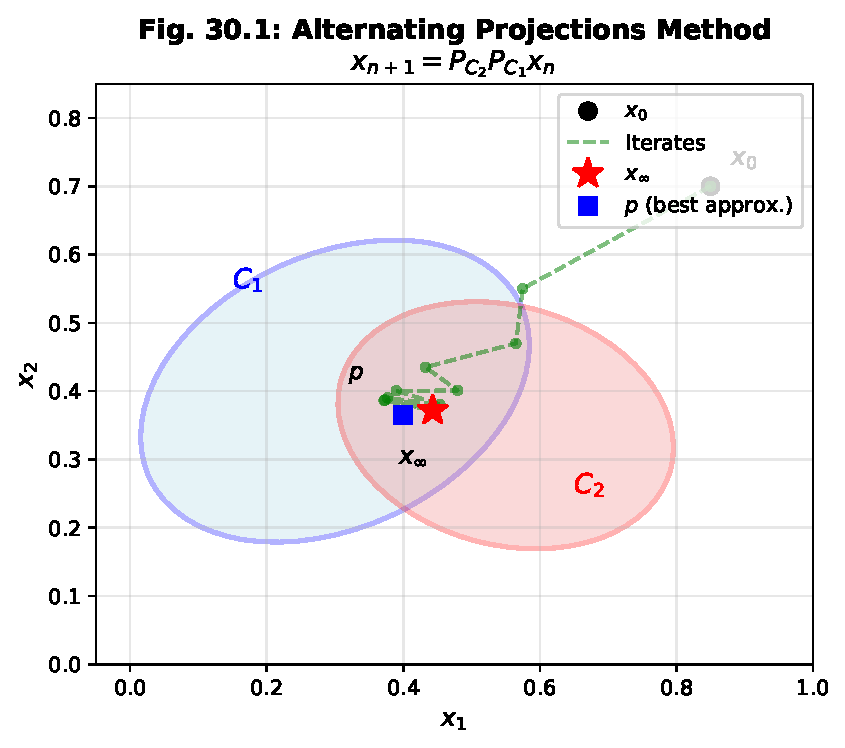
\includegraphics[width=0.4\textwidth]{fig_alternating_projections.pdf}
  \end{figure}
\end{frame}

% ============================================================================

\begin{frame}{Theorem 30.7: Dykstra's Algorithm}
  \begin{theorem}[Dykstra's Algorithm]
    Let $m$ be a strictly positive integer, set $I = \{1, \ldots, m\}$, let $(C_i)_{i \in I}$ be a family of closed convex subsets of $\mathcal{H}$ such that $C = \bigcap_{i \in I} C_i \neq \emptyset$, and let $x_0 \in \mathcal{H}$. Set
    \begin{align}
      i: \mathbb{N} \to I: n \mapsto 1 + \text{rem}(n-1, m),
    \end{align}
    where $\text{rem}(\cdot, m)$ is the remainder of division by $m$. For every strictly positive integer $n$, set $P_n = P_{C_{i(n)}}$ where $C_n = C_{i(n)}$ if $n > m$. Moreover, set $q_{-(m-1)} = \cdots = q_{-1} = q_0 = 0$ and
    \begin{align}
      \text{for } n = 1, 2, \ldots \quad
      \begin{cases}
        x_n = P_n(x_{n-1} + q_{n-m}) \\
        q_n = x_{n-1} + q_{n-m} - x_n
      \end{cases}
    \end{align}
    Then $x_n \to P_C x_0$.
  \end{theorem}
\end{frame}

% ============================================================================

\begin{frame}{Dykstra's Algorithm: Understanding the Recursion}
  The key variables are:
  \begin{itemize}
    \item $x_n$: the iterate (approximation to the projection)
    \item $q_n$: a residual/correction term
  \end{itemize}

  \vspace{0.3cm}

  The update can be understood as:
  \begin{align}
    x_n = P_{C_i(n)}(x_{n-1} + q_{n-m})
  \end{align}

  This means:
  \begin{enumerate}
    \item Add the accumulated correction from $m$ iterations ago
    \item Project onto the current set
    \item Record the projection residual as $q_n = (x_{n-1} + q_{n-m}) - x_n$
  \end{enumerate}

  \vspace{0.3cm}

  The corrections $q_n$ help the algorithm converge faster than simple alternating projections.
\end{frame}

% ============================================================================

\begin{frame}{Dykstra vs. Cyclic Projections}
  \begin{figure}
    \centering
    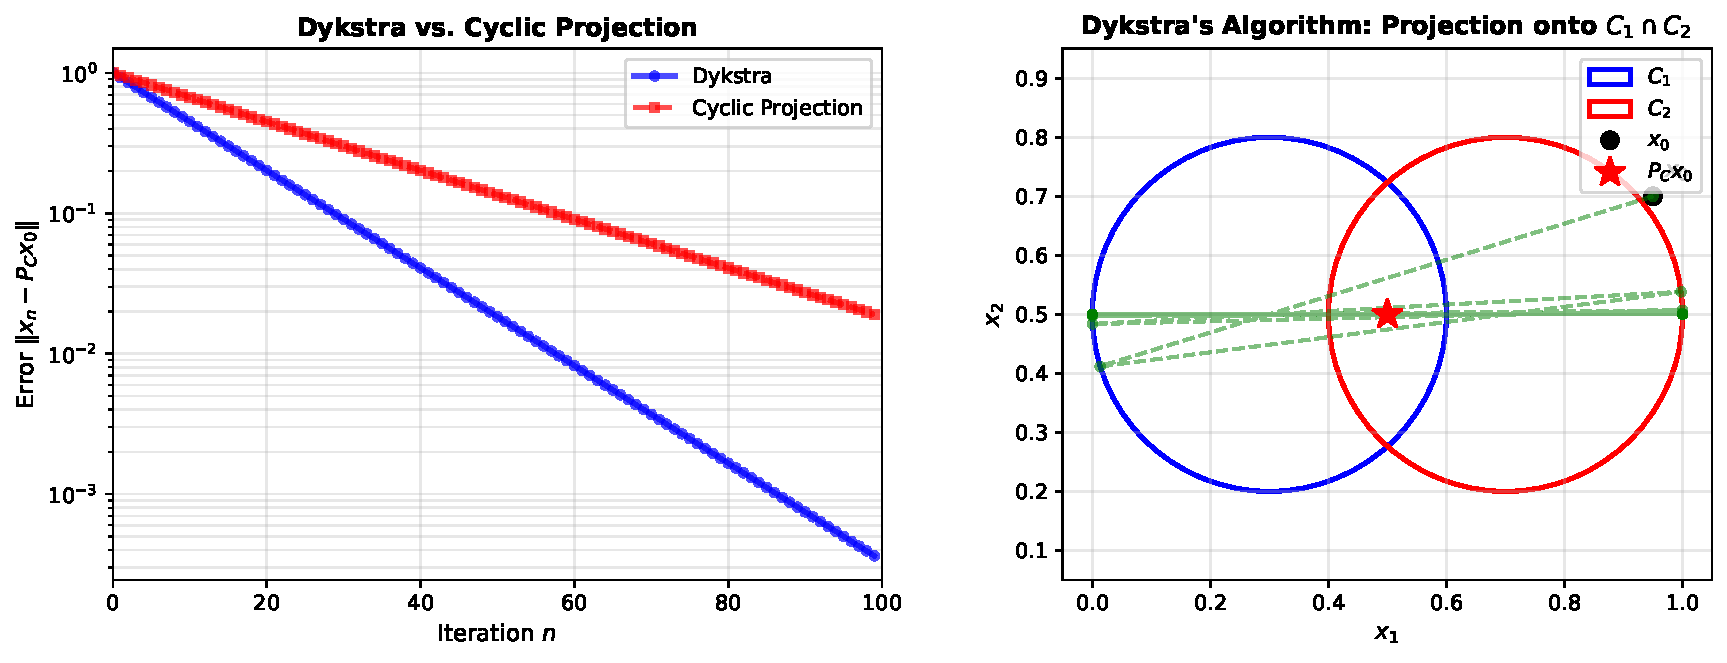
\includegraphics[width=0.8\textwidth]{fig_dykstra_convergence.pdf}
  \end{figure}

  \vspace{0.2cm}

  Key observation: Dykstra's algorithm converges faster than naive cyclic alternating projections due to the correction terms.
\end{frame}

% ============================================================================

\begin{frame}[fragile]{Dykstra's Algorithm: Python Implementation}
  \begin{lstlisting}
def dykstra_algorithm(projections, x0, m, max_iter=1000, tol=1e-8):
    """Dykstra's algorithm for projection onto intersection of m sets."""
    x = np.array(x0, dtype=float)
    q = [np.zeros_like(x) for _ in range(m)]
    history = [x.copy()]

    for n in range(1, max_iter + 1):
        # Index of current set (cyclic)
        i = (n - 1) % m

        # Dykstra step
        x_old = x.copy()
        if n <= m:
            correction = np.zeros_like(x)
        else:
            correction = q[(i - m) % m]

        x = projections[i](x + correction)
        q[i] = (x_old + correction) - x

        history.append(x.copy())
        if np.linalg.norm(x - x_old) < tol:
            break

    return x, np.array(history)
  \end{lstlisting}
\end{frame}

% ============================================================================

\begin{frame}{Corollary 30.4: Linear Mean Convergence for Dykstra}
  \begin{corollary}[Application to Two Sets]
    Consider the application of Dykstra's algorithm (Theorem 30.7) to $m = 2$ intersecting closed convex sets $C$ and $D$ of $\mathcal{H}$.
    \[
      \begin{cases}
        y_n = P_C(x_n + p_n) \\
        p_{n+1} = x_n + p_n - y_n \\
        x_{n+1} = P_D(y_n + q_n) \\
        q_{n+1} = y_n + q_n - x_{n+1}
      \end{cases}
    \]
    with $p_0 = q_0 = 0$. Then $x_n \to P_{C \cap D} x_0$ linearly.
  \end{corollary}

  \vspace{0.3cm}

  Advantages over alternating projections:
  \begin{enumerate}
    \item \textbf{Linear convergence} (not just weak convergence)
    \item \textbf{Exact} when sets are affine subspaces
    \item More efficient for practical problems
  \end{enumerate}
\end{frame}

% ============================================================================
\section{Haugazeau's Algorithm}
% ============================================================================

\begin{frame}{Haugazeau's Algorithm: Motivation}
  \begin{block}{Extension of Dykstra}
    Haugazeau's algorithm generalizes Dykstra's approach to handle:
    \begin{itemize}
      \item Families of \textbf{firmly quasinonexpansive} operators (more general than projections)
      \item Cyclic application of operators
      \item Non-cyclic scheduling
    \end{itemize}
  \end{block}

  \vspace{0.3cm}

  Application areas:
  \begin{enumerate}
    \item Projection onto intersections of convex sets
    \item Minimizing sums of convex functions
    \item Solving operator equations and inclusions
  \end{enumerate}
\end{frame}

% ============================================================================

\begin{frame}{Theorem 30.8: Haugazeau's Algorithm}
  \begin{theorem}[Haugazeau's Algorithm]
    Let $(T_i)_{i \in I}$ be a finite family of firmly quasinonexpansive operators from $\mathcal{H}$ to $\mathcal{H}$ such that the operators $(\text{Id} - T_i)_{i \in I}$ are demiclosed at 0 and $C = \bigcap_{i \in I} \text{Fix } T_i \neq \emptyset$. Let $x_0 \in \mathcal{H}$. Let $i: \mathbb{N} \to I$ be such that there exists a strictly positive integer $m$ for which
    \[
      (\forall i \in I)(\forall n \in \mathbb{N}) \quad i \in \{i(n), \ldots, i(n+m-1)\},
    \]
    and set
    \[
      (\forall n \in \mathbb{N}) \quad x_{n+1} = Q(x_0, x_n, T_{i(n)} x_n),
    \]
    where $Q$ is defined in Theorem 29.39. Then $x_n \to P_C x_0$.
  \end{theorem}

  \vspace{0.3cm}

  Key assumption: \textbf{Cyclic scheduling} - each operator is applied regularly (at least once every $m$ iterations).
\end{frame}

% ============================================================================

\begin{frame}{Haugazeau's Algorithm: Visualization}
  \begin{figure}
    \centering
    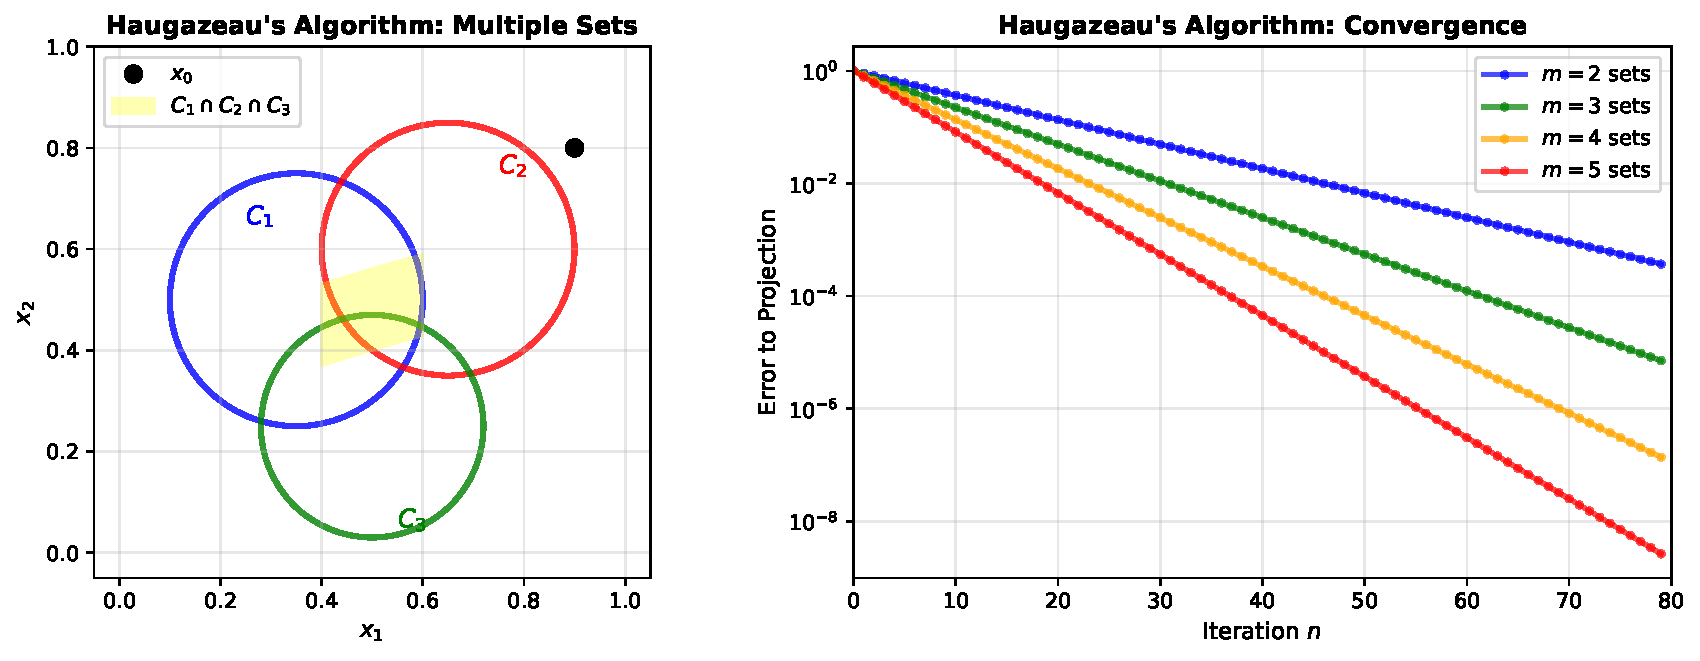
\includegraphics[width=0.8\textwidth]{fig_haugazeau_algorithm.pdf}
  \end{figure}

  The algorithm handles multiple sets and converges to their intersection.
\end{frame}

% ============================================================================

\begin{frame}{Corollary 30.9: Finite Family of Continuous Convex Functions}
  \begin{corollary}
    Let $(f_i)_{i \in I}$ be a finite family of continuous convex functions from $\mathcal{H}$ to $\mathbb{R}$ such that $C = \bigcap_{i \in I} \text{lev}_{\leq 0} f_i \neq \emptyset$ and suppose that one of the following holds:
    \begin{enumerate}
      \item[(i)] The functions $(f_i)_{i \in I}$ are bounded on every bounded subset of $\mathcal{H}$.
      \item[(ii)] The functions $(f_i)^*_{i \in I}$ are supercoercive.
      \item[(iii)] $\mathcal{H}$ is finite-dimensional.
    \end{enumerate}
    Then $x_n \to P_C x_0$ via Algorithm 30.64.
  \end{corollary}

  \vspace{0.3cm}

  This applies Haugazeau's algorithm to feasibility problems for systems of convex inequalities.
\end{frame}

% ============================================================================

\begin{frame}{Corollary 30.10: Firmly Nonexpansive Operators}
  \begin{corollary}
    Let $(T_i)_{i \in I}$ be a finite family of firmly nonexpansive operators from $\mathcal{H}$ to $\mathcal{H}$ such that $C = \bigcap_{i \in I} \text{Fix } T_i \neq \emptyset$. Let $x_0 \in \mathcal{H}$, let $i: \mathbb{N} \to I$ be such that there exists a strictly positive integer $m$ for which
    \[
      (\forall i \in I)(\forall n \in \mathbb{N}) \quad i \in \{i(n), \ldots, i(n+m-1)\},
    \]
    and set
    \[
      (\forall n \in \mathbb{N}) \quad x_{n+1} = Q(x_0, x_n, T_{i(n)} x_n),
    \]
    where $Q$ is defined in (29.39). Then $x_n \to P_C x_0$.
  \end{corollary}

  Note: Firmly nonexpansive operators include projections onto convex sets.
\end{frame}

% ============================================================================

\begin{frame}{Corollary 30.11: Proximal Point Algorithm for Maximally Monotone Operators}
  \begin{corollary}
    Let $A: \mathcal{H} \to 2^{\mathcal{H}}$ be maximally monotone and such that $0 \in A x_0$ and let $x_0 \in \mathcal{H}$. Let $J_A = (\text{Id} + A)^{-1}$ (the resolvent). Set
    \[
      (\forall n \in \mathbb{N}) \quad x_{n+1} = Q(x_0, x_n, J_A x_n),
    \]
    where $Q$ is defined in (29.39). Then $x_n \to P_{\text{zer } A} x_0$.
  \end{corollary}

  \vspace{0.3cm}

  \textbf{Key result}: The proximal point algorithm finds zeros of maximally monotone operators with strong convergence.

  \vspace{0.3cm}

  Applications: Subgradient methods, splitting algorithms, monotone inclusion problems.
\end{frame}

% ============================================================================

\begin{frame}{Corollary 30.12: Forward-Backward Algorithm}
  \begin{corollary}
    Let $A: \mathcal{H} \to 2^{\mathcal{H}}$ be maximally monotone, let $\beta \in \mathbb{R}_{++}$, let $B: \mathcal{H} \to \mathcal{H}$ be $\beta$-cocoercive, and let $\gamma \in [0, 2\beta]$. Suppose that $\text{zer}(A + B) \neq \emptyset$. Let $x_0 \in \mathcal{H}$ and set
    \begin{align}
      \text{for } n = 0, 1, \ldots \quad
      \begin{cases}
        y_n = x_n - \gamma B x_n \\
        z_n = (1/2)(x_n + J_{\lambda A} y_n) \\
        x_{n+1} = Q(x_0, x_n, z_n)
      \end{cases}
    \end{align}
    where $Q$ is defined in (29.39). Then $x_n \to P_{\text{zer}(A+B)} x_0$.
  \end{corollary}

  \vspace{0.3cm}

  \begin{itemize}
    \item Handles sum of maximally monotone and cocoercive operators
    \item Splits the computation of resolvents
  \end{itemize}
\end{frame}

% ============================================================================

\begin{frame}{Example 30.13: Composite Optimization}
  \begin{example}
    Let $f \in \Gamma_0(\mathcal{H})$, let $\beta \in \mathbb{R}_{++}$, let $g: \mathcal{H} \to \mathbb{R}$ be convex and differentiable with $1/\beta$-Lipschitz continuous gradient, and let $\gamma \in [0, 2\beta]$. Furthermore, suppose that $\text{Argmin}(f + g) \neq \emptyset$. Let $x_0 \in \mathcal{H}$ and set
    \begin{align}
      \text{for } n = 0, 1, \ldots \quad
      \begin{cases}
        y_n = x_n - \gamma \nabla g(x_n) \\
        z_n = (1/2)(x_n + \text{Prox}_{f} y_n) \\
        x_{n+1} = Q(x_0, x_n, z_n)
      \end{cases}
    \end{align}
    where $Q$ is defined in (29.39). Then $x_n \to P_{\text{Argmin}(f+g)} x_0$.
  \end{example}

  \vspace{0.3cm}

  \textbf{Interpretation}: Forward-backward splitting for minimizing sum of smooth and nonsmooth convex functions.
\end{frame}

% ============================================================================

\begin{frame}{Summary: Algorithm Comparison}
  \begin{table}
    \centering
    \begin{tabular}{|l|c|c|c|}
      \hline
      \textbf{Algorithm} & \textbf{Convergence} & \textbf{Operators} & \textbf{Complexity} \\
      \hline
      Halper's & Weak & Any nonexp. & Low \\
      \hline
      Dykstra's & Linear & Projections & Low \\
      \hline
      Haugazeau's & Strong & Firmly quasi-nonexp. & Medium \\
      \hline
      Proximal Pt. & Strong & Maximally monotone & High \\
      \hline
      Forward-Backward & Strong & $A$ + $B$ composite & Medium \\
      \hline
    \end{tabular}
  \end{table}

  \vspace{0.3cm}

  Convergence hierarchy: Weak < Linear < Strong convergence
\end{frame}

% ============================================================================
\section{Applications and Numerical Examples}
% ============================================================================

\begin{frame}{Projections onto Common Convex Sets}
  \begin{figure}
    \centering
    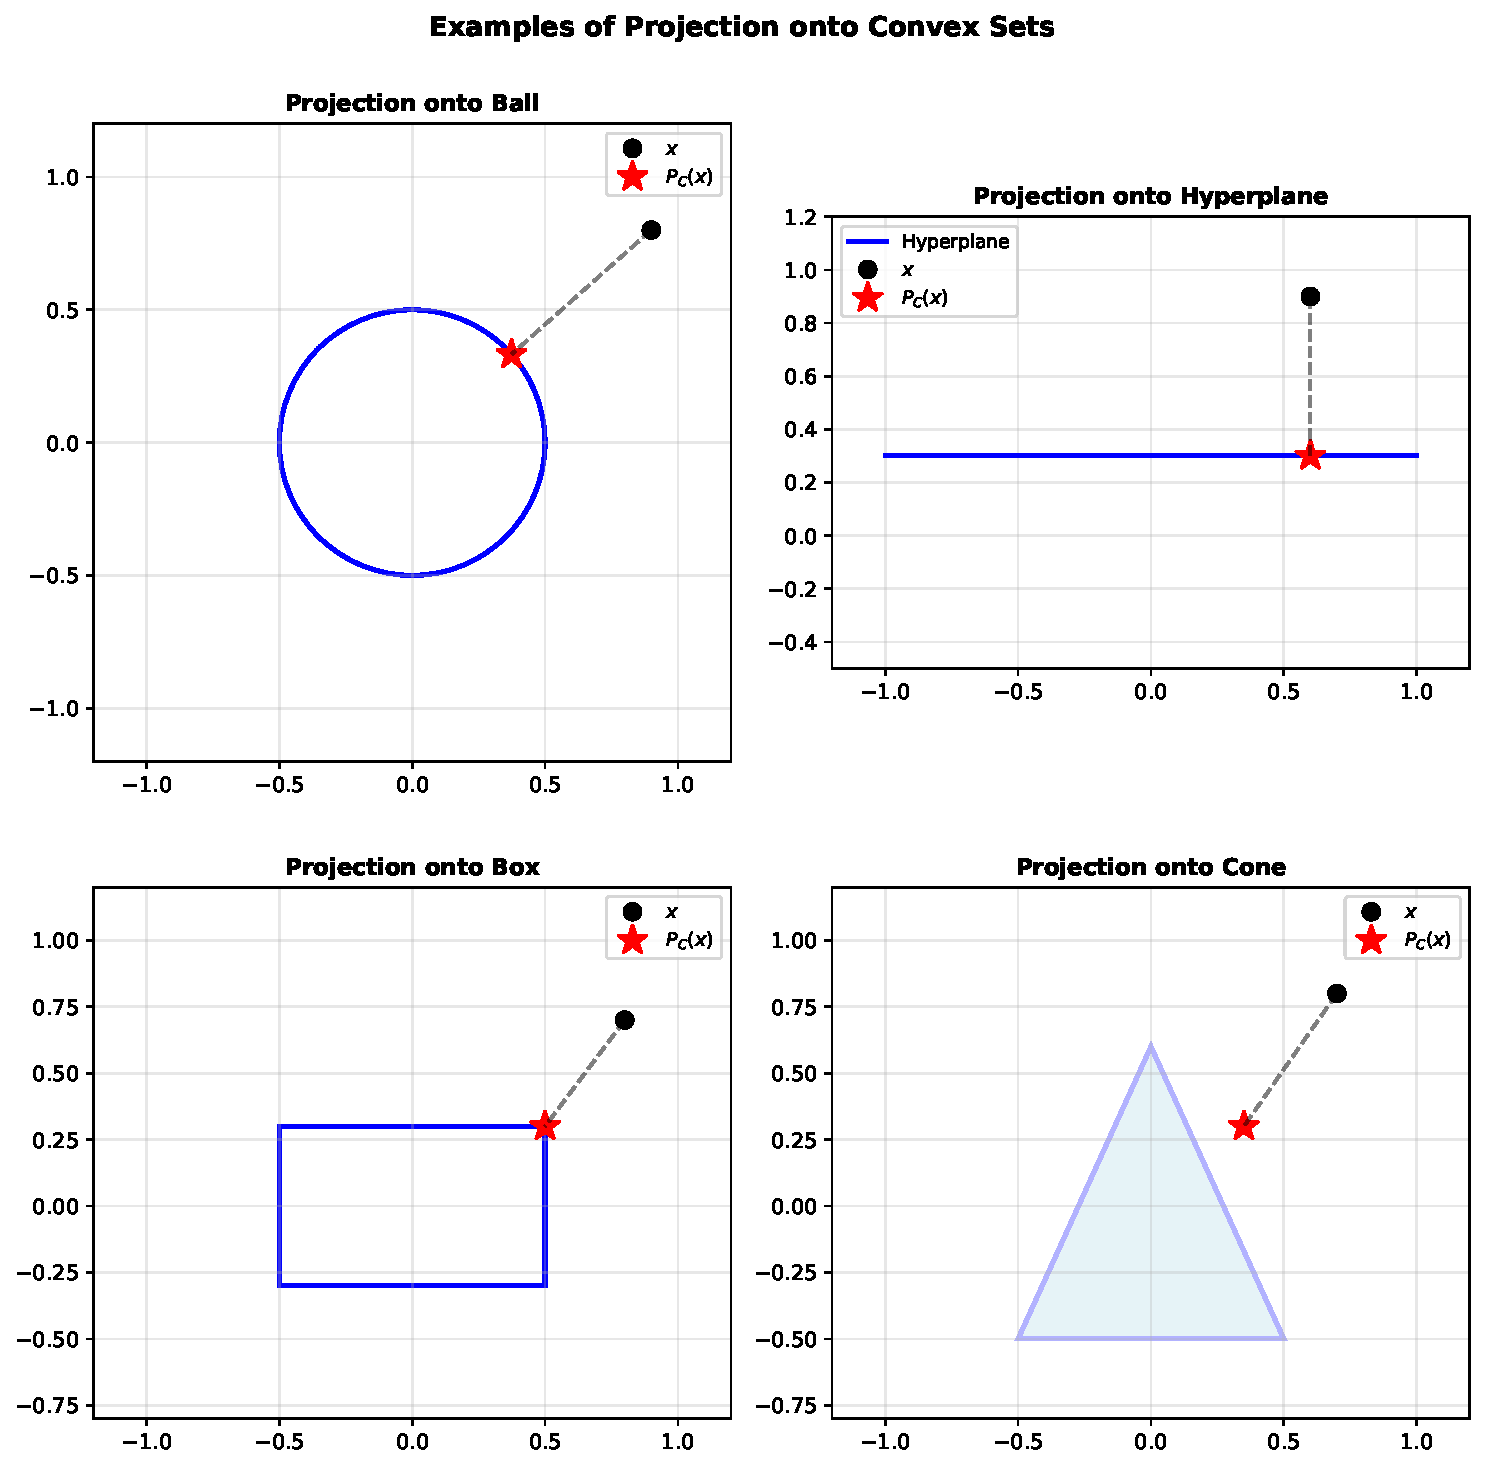
\includegraphics[width=0.9\textwidth]{fig_projections.pdf}
  \end{figure}

  Each has a simple closed form:
  \begin{itemize}
    \item Ball: Radial scaling
    \item Hyperplane: Orthogonal projection
    \item Box: Componentwise clipping
    \item Cone: Convex cone projection
  \end{itemize}
\end{frame}

% ============================================================================

\begin{frame}{Numerical Convergence Rates}
  \begin{figure}
    \centering
    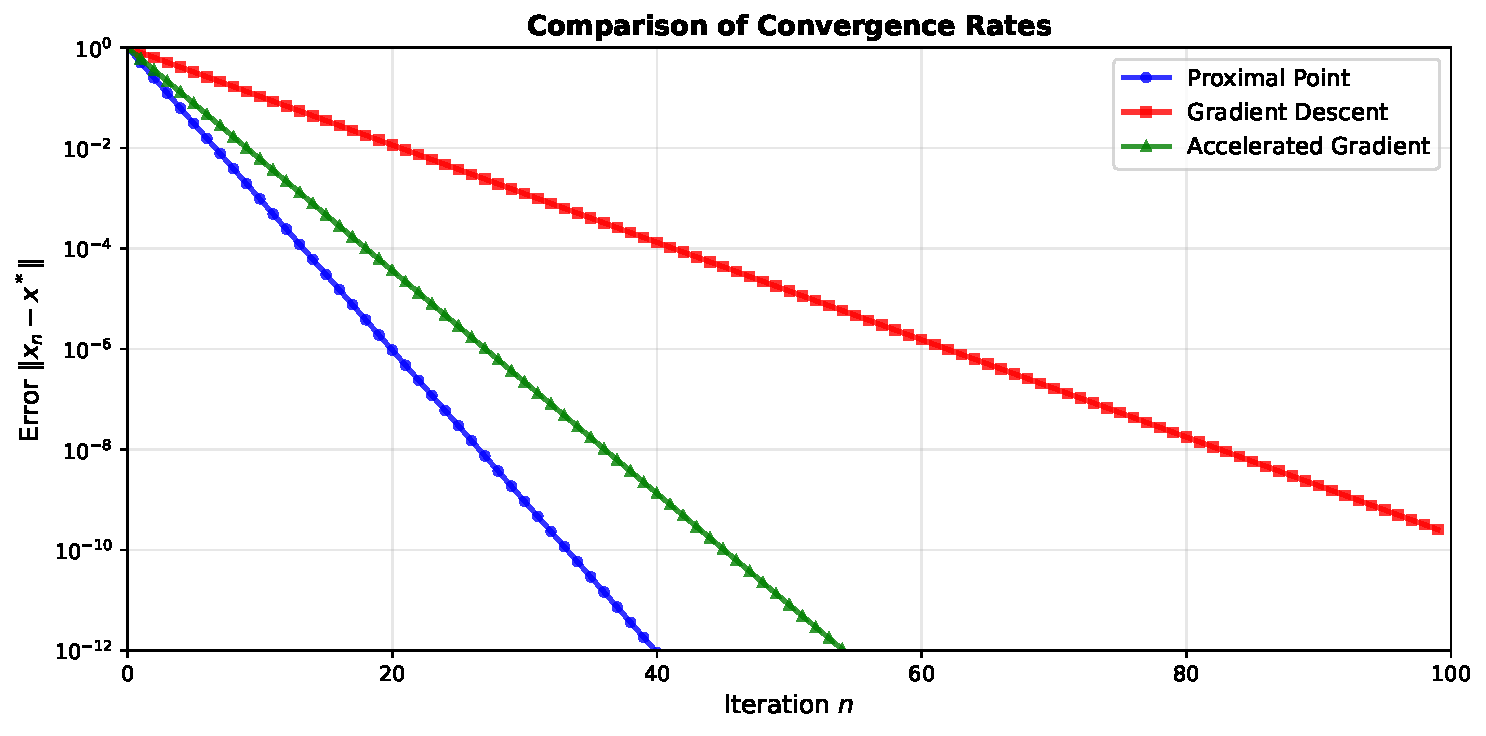
\includegraphics[width=0.9\textwidth]{fig_proximal_point.pdf}
  \end{figure}

  \vspace{0.2cm}

  Comparison of standard first-order methods for convex optimization.
\end{frame}

% ============================================================================

\begin{frame}[fragile]{Example: Projection onto Intersection of Two Disks}
  \begin{lstlisting}
import numpy as np

# Define two circular sets
C1_center, C1_radius = np.array([0.3, 0.5]), 0.3
C2_center, C2_radius = np.array([0.7, 0.5]), 0.3

def proj_C1(x):
    d = np.linalg.norm(x - C1_center)
    if d <= C1_radius:
        return x
    return C1_center + C1_radius * (x - C1_center) / d

def proj_C2(x):
    d = np.linalg.norm(x - C2_center)
    if d <= C2_radius:
        return x
    return C2_center + C2_radius * (x - C2_center) / d

# Initial point
x0 = np.array([0.95, 0.7])

# Dykstra's algorithm
m = 2
projections = [proj_C1, proj_C2]
x_final, history = dykstra_algorithm(projections, x0, m)

print(f"Initial point: {x0}")
print(f"Projection: {x_final}")
print(f"Iterations: {len(history)}")
  \end{lstlisting}
\end{frame}

% ============================================================================

\begin{frame}{Convergence Illustration}
  \begin{figure}
    \centering
    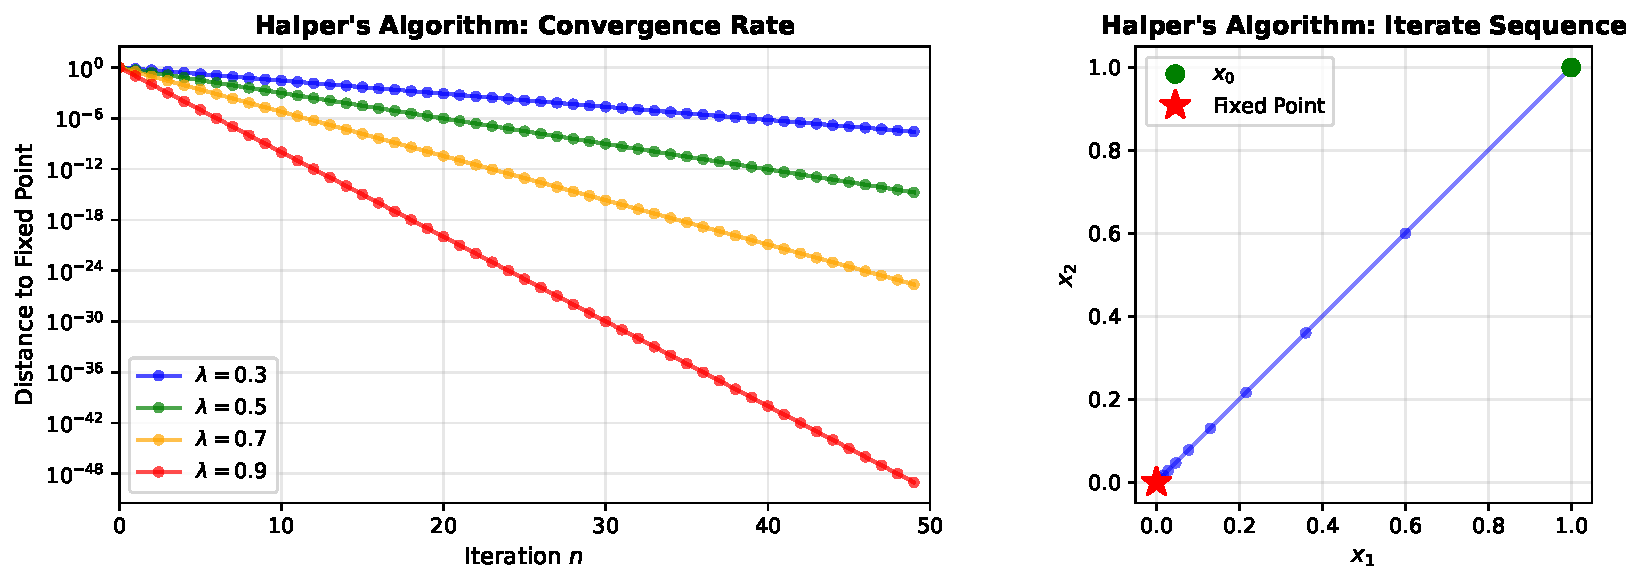
\includegraphics[width=0.9\textwidth]{fig_halpers_convergence.pdf}
  \end{figure}

  Left: Theoretical convergence rates depend on the parameter $\lambda$.
  Right: Iterates converge to the fixed point.
\end{frame}

% ============================================================================

\begin{frame}{Forward-Backward Splitting Example}
  \begin{figure}
    \centering
    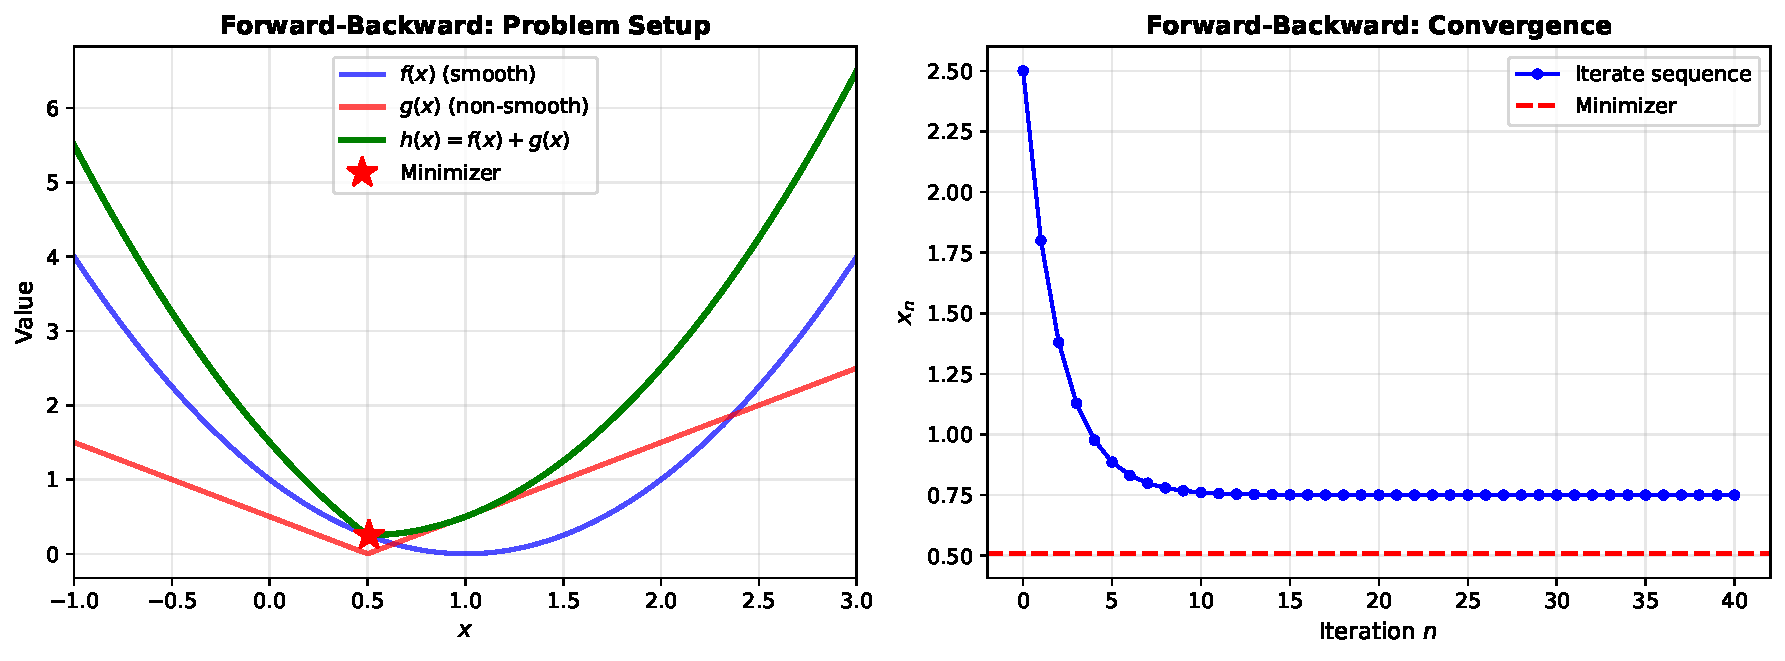
\includegraphics[width=0.9\textwidth]{fig_forward_backward.pdf}
  \end{figure}

  Left: Problem setup (smooth + nonsmooth objective).
  Right: Convergence of iterates to minimizer.
\end{frame}

% ============================================================================
\section{Key Theoretical Results}
% ============================================================================

\begin{frame}{Demiclosedness and Quasinonexpansiveness}
  \begin{definition}[Demiclosed at 0]
    An operator $T: \mathcal{H} \to \mathcal{H}$ is \textbf{demiclosed at 0} if whenever $(x_n)_n$ is a sequence with $x_n \to x$ weakly and $(I - T)x_n \to 0$ strongly, then $(I - T)x = 0$.
  \end{definition}

  \vspace{0.3cm}

  \begin{definition}[Firmly Quasinonexpansive]
    An operator $T: \mathcal{H} \to \mathcal{H}$ is \textbf{firmly quasinonexpansive} if
    \begin{align}
      \text{Fix } T = \{x : Tx = x\} \neq \emptyset \quad \text{and} \quad
      \|Tx - Ty\|^2 + \|Tx - y\|^2 \leq \|x - y\|^2, \quad \forall x, y \in \mathcal{H}.
    \end{align}
  \end{definition}

  \vspace{0.3cm}

  \textbf{Key fact}: Projections are firmly nonexpansive and demiclosed.
\end{frame}

% ============================================================================

\begin{frame}{Lemmata for Convergence Analysis}
  \begin{lemma}[30.6: Cauchy-Schwarz for Sequences]
    Let $(\rho_n)_n \in \ell_2^2(\mathbb{N})$, let $m \in \mathbb{N}$, and set $(\forall n \in \mathbb{N}) \sigma_n = \sum_{k=0}^{n} \rho_k$. Then
    \[
      \lim \sigma_n(\sigma_n - \sigma_{n-m-1}) = 0.
    \]
  \end{lemma}

  \vspace{0.3cm}

  This is a key tool for analyzing the residuals in Dykstra's algorithm.

  \vspace{0.3cm}

  \begin{lemma}
    The residual terms $q_n$ in Dykstra's algorithm satisfy:
    \begin{itemize}
      \item They are bounded: $\sum_k \|q_k\|^2 < \infty$
      \item They converge to zero: $q_n \to 0$
      \item This ensures convergence to the fixed point
    \end{itemize}
  \end{lemma}
\end{frame}

% ============================================================================

\begin{frame}{Remark 30.14: Connection to Fixed Point Methods}
  \begin{remark}
    The principle employed in the proof of Corollary 30.12 is general:

    Let $(R_i)_{i \in I}$ be a finite family of nonexpansive operators from $\mathcal{H}$ to $\mathcal{H}$ such that $\bigcap_{i \in I} \text{Fix } R_i \neq \emptyset$ and set $(\forall i \in I) T_i = (1/2)(R_i + \text{Id})$.

    Then $\bigcap_i \text{Fix } T_i = \bigcap_i \text{Fix } R_i$, and it follows from Proposition 4.4 that the operators $(T_i)_{i \in I}$ are firmly nonexpansive.

    Thus, Theorem 30.8 can be used to find the best approximation to a point $x_0 \in \mathcal{H}$ from $\bigcap_i \text{Fix } R_i$.
  \end{remark}

  \vspace{0.3cm}

  This shows that firmly nonexpansive methods are a unifying framework.
\end{frame}

% ============================================================================

\begin{frame}{Corollary 30.15: Haugazeau's Algorithm (Cyclic Version)}
  \begin{corollary}[Haugazeau's Algorithm - Cyclic Projections]
    Let $m$ be a strictly positive integer, set $I = \{1, \ldots, m\}$, let $(C_i)_{i \in I}$ be a family of closed convex subsets of $\mathcal{H}$ such that $C = \bigcap_{i \in I} C_i \neq \emptyset$, and let $x_0 \in \mathcal{H}$. For every $i \in I$, denote by $P_i$ the projector onto $C_i$. Let $\text{rem}(\cdot, m)$ be the remainder function of division by $m$, and set
    \[
      (\forall n \in \mathbb{N}) \quad x_{n+1} = Q(x_0, x_n, P_{1+\text{rem}(n,m)} x_n),
    \]
    where $Q$ is defined in (29.39). Then $x_n \to P_C x_0$.
  \end{corollary}

  \vspace{0.3cm}

  This is the complete cyclic projection algorithm using Haugazeau's framework.
\end{frame}

% ============================================================================
\section{Exercises and Further Reading}
% ============================================================================

\begin{frame}{Selected Exercises}
  \begin{exercise}[30.1]
    Suppose that $\mathcal{H} = \mathbb{R}$, and set $D = [-1, 1]$, $x = 0$, and $x_0 = 1$. By considering $T_1: D \to D: x \mapsto 1$ and $T_2: D \to D: x \mapsto -x$, show that Theorem 30.1 fails when (i) or (ii) is not satisfied.
  \end{exercise}

  \vspace{0.3cm}

  \begin{exercise}[30.2]
    Give a detailed proof of Corollary 30.5 (Linear Mean Ergodic Theorem).
  \end{exercise}

  \vspace{0.3cm}

  \begin{exercise}[30.4(ii)]
    Consider the application of Dykstra's algorithm to $m = 2$ intersecting closed convex subsets $C$ and $D$ of $\mathbb{R}^2$. With $H = \mathbb{R}^2$, $x_0 = (2, 2)$, $C = \{(\xi_1, \xi_2) \in \mathcal{H} \mid \xi_2 \leq 0\}$, $D = \{(\xi_1, \xi_2) \in \mathcal{H} \mid \xi_1 + \xi_2 \leq 0\}$. Compute the values of $x_n$ for $n \in \{0, \ldots, 5\}$ and draw a picture.
  \end{exercise}
\end{frame}

% ============================================================================

\begin{frame}{Key Takeaways}
  \begin{enumerate}
    \item \textbf{Halper's Algorithm}: Solves the best approximation problem using convex combinations of operator iterates with decaying step sizes.

    \vspace{0.3cm}

    \item \textbf{Dykstra's Algorithm}: Specialized for projections onto intersections of convex sets; uses residual corrections for linear convergence.

    \vspace{0.3cm}

    \item \textbf{Haugazeau's Algorithm}: General framework for firmly quasinonexpansive operators; includes proximal point and forward-backward splitting.

    \vspace{0.3cm}

    \item \textbf{Convergence Theory}: Relies on demiclosedness, weak convergence subsequences, and properties of monotone operators.

    \vspace{0.3cm}

    \item \textbf{Applications}: Feasibility, convex optimization, monotone inclusions, machine learning algorithms.
  \end{enumerate}
\end{frame}

% ============================================================================

\begin{frame}{References}
  \begin{itemize}
    \item Bauschke, H. H., \& Combettes, P. L. (2017). \textit{Convex Analysis and Monotone Operator Theory in Hilbert Spaces} (2nd ed.). Springer.

    \vspace{0.2cm}

    \item Chapter 30: Best Approximation Algorithms (pp. 991--1032)
      \begin{itemize}
        \item Sections 30.1--30.3: Halper's, Dykstra's, and Haugazeau's algorithms
        \item Applications to projections, monotone inclusions, and convex optimization
      \end{itemize}

    \vspace{0.2cm}

    \item Related chapters:
      \begin{itemize}
        \item Chapter 4: Convexity, monotonicity, and firm nonexpansivity
        \item Chapter 5: Convergence of sequences
        \item Chapter 29: Monotone operators and resolvents
      \end{itemize}
  \end{itemize}
\end{frame}

% ============================================================================

\begin{frame}[allowframebreaks]{Summary of Theorems and Corollaries}
  \begin{itemize}
    \item \textbf{Theorem 30.1}: Halper's Algorithm - basic convergence
    \item \textbf{Corollary 30.2}: Weighted combination of operators
    \item \textbf{Corollary 30.3}: Composite averaged nonexpansive operators
    \item \textbf{Corollary 30.5}: Linear Mean Ergodic Theorem
    \item \textbf{Theorem 30.7}: Dykstra's Algorithm - cyclic projections
    \item \textbf{Theorem 30.8}: Haugazeau's Algorithm - general framework
    \item \textbf{Corollary 30.9}: Finite family of convex functions
    \item \textbf{Corollary 30.10}: Firmly nonexpansive operators
    \item \textbf{Corollary 30.11}: Proximal Point Algorithm
    \item \textbf{Corollary 30.12}: Forward-Backward Splitting
    \item \textbf{Corollary 30.15}: Haugazeau's Algorithm (Cyclic)
  \end{itemize}

  \vspace{0.3cm}

  All algorithms share common features:
  \begin{itemize}
    \item Iteration based on simple operations (projections, resolvents)
    \item Convergence guaranteed under appropriate conditions
    \item Applicable to diverse optimization and operator problems
  \end{itemize}
\end{frame}

% ============================================================================

\end{document}
